\section{Hiding Routing Information}
    \subsection{Wprowadzenie}
        \begin{itemize}
            \item Ogranicza podatności sieci na analizę ruchu sieciowego
            \item Ukrywa informacje dotyczące routowania
        \end{itemize}

    \subsection{Cebule}
        \begin{itemize}
            \item W celu rozpoczęcia sesji pomiędzy inicjatorem i~odbiorcą, proxy inicjatora identyfikuje serie węzłów routujących, które tworzą ścieżkę przez sieć i~tworzą \textit{cebulę}, która enkapsuluje tą sieżkę.
            \item Rysunek przedstawia cebulę skonstruowaną przez węzeł Proxy/Routujący W, do węzła Proxy/Routującego Z. Ścieżka przechodzi przez węzły X, oraz Z.
            \begin{figure}
                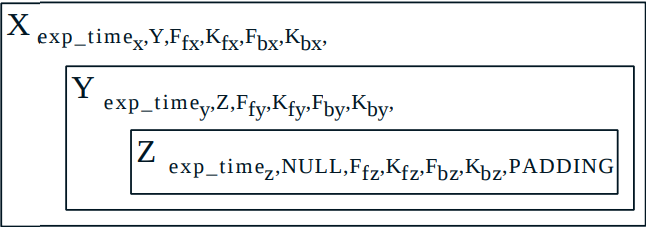
\includegraphics[width=\textwidth]{onion}
            \end{figure}
            \item Cały proces trasowania cebulowego (W --> X --> Y --> Z)
            \begin{itemize}
                \item Struktura cebuli (kolejność warstw szyfru, kolejność węzłów, itd.)
                \item Każdy węzeł wie kto przysłał mu wiadomość do kogo ma trafić, ale nie zna źródła i~celu samej wiadomości
                \item Rysunek przedstawia format wiadomości otrzymanej przez węzeł $P_x$. 
                
                $\{exp\_time, next\_hop, F_f, K_f, F_b, K_b, payload\}_{PK_x}$, gdzie $PK_x$ jest kluczem publicznym węzła $P_x$, który posiada klucz deszyfrujący, exp\_time to czas wygaśnięcia cebuli.

                \item Wiadomość jaką otrzymuje węzeł $P_x$ wygląda następująco

                $\{ exp\_time, next\_hop, F_f, K_f, F_b, K_b, payload \}_{PK_x}$
                \begin{itemize}
                    \item $PK_x$ szyfrujący klucz publiczny węzła $P_x$
                    \item $exp\_time$ - czas wygaśnięcia cebuli, używany w~celu wykrycia 
                    \item następny węzeł do którego mają trafić dane
                    \item dane
                    \item dwie pary funkcji/kluczy, określających operacje kryptograficzne i klucze, które mają być zastosowane do danych przesyłanych przez wirtualny obwód. Para $(F_f, K_f)$ jest zastosowana do danych przechodzących na przód, a~para $(F_b, K_b)$ jest zasotosowana do przeciwnego kierunku.
                \end{itemize}
                \item Każdy przeskok pomniejsza cebulę poprzez zdjęcie z~niej warstwy. Aby uniknąć wykrycia miejsca węzła w~trasie, na końcu danych umieszcza się losowy ciąg bitów o~wielkości zdjętej warstwy, przed wysłaniem wiadomości do następnego węzła. Dzięki temu tylko ostatni węzeł wie jak duże jest dopełnienie wiadomości, ponieważ znajduje się na końcu trasy i~o~tym wie.
            \end{itemize}
        \end{itemize}

        \begin{figure}
            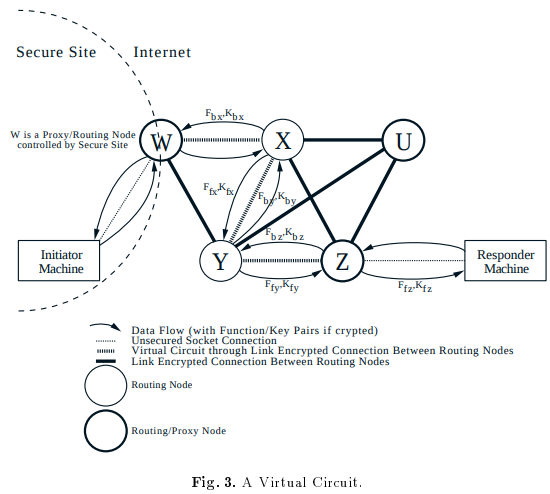
\includegraphics[width=\textwidth]{wirtualny_obwod}
        \end{figure}
        \subsection{Tworzenie obwodu}
        \begin{itemize}
            \item Wiadomość zawiera id obwodu, komendę (create, destroy i data), oraz dane
            \item Węzeł, który otrzyma wiadomość zawierającą komendę \textit{create} wybiera id wirtualnego obwodu i wysyła kolejną wiadomość \textit{create} zawierającą ten id do następnego węzła. Węzeł przechowuje id wirtualnego obwodu, który otrzymał i~id wirtualnego obwodu jaki wysłał, jako parę.
            \item funkcja kryptograficzna i~klucz kryptograficzny są stosowane do danych przesyłanych w~przód obwodu, oraz w~przeciwnym kierunku. Dla każdego kierunku stosowane są oddzielne pary funkcja/klucz.
            \item rysunek 3. przedstawia wirtualny obwod dla cebuli widocznej na rysunku 2.
            \item Proxy inicjatora szyfruje wysyłaną wiadomość stosując odwrotną kolejność operacji kryptograficznych. Wiadomość znajduje się najgłębiej w~cebuli.
        \end{itemize}
        \subsection{Luźny routing}
        \begin{itemize}
            \item Proxy inicjatora nie musi okereślać całej ścieżki. Zamiast tego nakazać konkretnemu węzłowi, aby ten sam wybrał trasę do następnego węzła. Dzięki temu w obwodzie znajduje się więcej przeskoków, co ma wpływ na wzrost bezpieczeństwa. Jeśli proxy inicjatora nie zna kompletnej ścieżki do punktu docelowego, wtedy węzeł może zbudować ścieżkę do następnego węzła. Luźny routing może być wykorzystany obsługi zmian połączenia, krórego proxy inicjatora nie jest świadomy.
            \item Możliwe jest również zezwolenie węzłom w~dodanej ścieżce na użycie tego procesu, ale potrzebny jest mechanizm, który ochroniłby przed tworzeniem ścieżki o~nieskończonej długości. Cebula, która pozwala na użycie luźnego routingu wygląda następująco:

            $\{exp\_time, next\_hop, max\_loosecount, F_f, K_f, F_b, K_b, payload\}_{PK_x}$

            \item Jeśli węzeł, który odbierze cebulę, zadecyduje o~użyciu luźnego routingu, przygotowuje nową cebulę z~maksymalnie max\_loosecount ilością warstw. Danymi w tej cebuli jest po prostu odebrana cebula ze zmienionym $PK_x$ dla ostatniego (najgłębszego) węzła, którego dodał do łańcucha. Innymi słowy zachowuje się on jak proxy inicjatora, z~tym wyjątkiem, że przesyłane w~cebuli dane są również cebulą. W celu utrzymania stałej długości cebuli, węzeł musi obciąć ilość danych współmierną do ilości dodanych warstw. Inicjujące proxy musi przewidzieć ilość dopełnienia (zarówno obecnego początkowo, jak i~każdego dodanego i/lub obciętego podczas przechodzenia przez ścieżkę), które będzie występować w~centralnych danych podczas trwania luźnego routingu, które będzie zezwalać na to obcięcie. Całkowita wartość wszystkich max\_loosesount występujących w~dodanych warstwach plus liczba dodanych warstw musi być mniejsza lub równa wartości max\_loosecount odebranej przez dodany węzeł.
        \end{itemize}

        \begin{figure}
            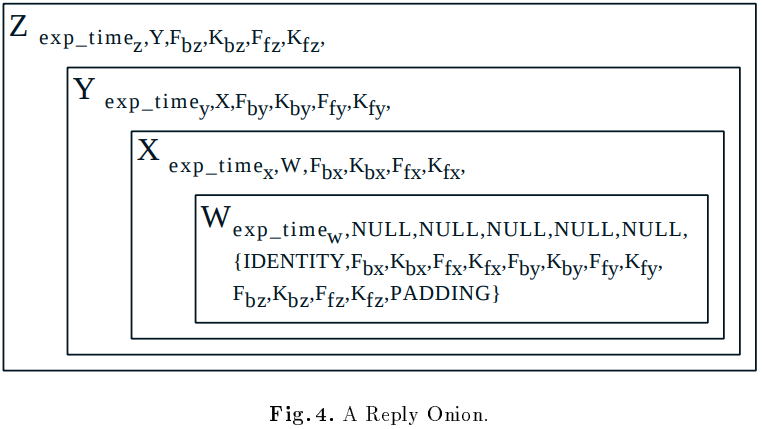
\includegraphics[width=\textwidth]{reply_onion}
        \end{figure}
        \subsection{Cebule zwrotne}
        \begin{itemize}
            \item W~niektórych aplikacjach przydatne jest odsyłanie wiadomości zwrotnych (odpowiedzi, ang. replay) przez serwer docelowy, podczas uszkodzenia oryginalnego obwodu. To pozwoliłoby na wysyłanie odpowiedzi (np. email) na zapytania, które nie były dostępne podczas oryginalnego połączenia. Jak teraz zobaczymy, to również pozwala odbiorcy, tak samo jak nadawcy, na pozostanie ukrytym.
            \item Cebule zwrotne mają taką samą strukturę jak zwykłe cebule, a~węzły traktują je w~ten sam sposób.
            \item Główną różnicą między cebulą zwykłą (przekazującą, ang. forward), a~odpowiadającą (ang. reply) jest najgłębsza treść. W~cebuli przekazującej może być ona pusta (zawierająca jedynie padding (dopełnienie)). Treść cebuli zwrotnej zawiera wystarczającą ilość informacji, aby umożliwić proxy inicjatora dotarcie do inicjatora i~wszystkich par funkcji kryptograficznych i kluczy z~cebuli.
            \item Rysunek 4. przedstawia cebulę zwrotną skonstruowaną przez Węzeł Proxy/Router W inicjatora.
            \item Zwrotna trasa rozpoczyna się w Węźle Proxy/Routerze Z odbiorcy przez pośrednie węzły routujące Y, oraz X.
            \item Przekierowywujące funkcje kryptograficzne są przypisane do danych poruszających się w~kierunku, w~którym obwód został ustanowiony.
            \item Kryptograficzne funkcje zwrotne są przypisane do danych poruszających się w przeciwnym kierunku
            \item Lokalizacja końcowych Węzłów Proxy/Routujących jest odwrócona. (inicjator na końcu, odbiorca na początku)
            \item Zarówno cebula przekierowująca jak i~zwrotna może być użyta tylko raz. Kiedy węzeł odbierze cebulę, utrzymuje ją aż do momentu wygaśnięcia. Każda odebrana cebula jest z~nią porównywana w~celu wykrycia powtórek, które są traktowane jako błędne i~są ignorowane. 
        \end{itemize}
        
        \subsection{Implementacja}
	\begin{itemize}
	  \item Wprowadzenie
	  \begin{itemize}
	  \item Tradycyjny serwer proxy działa na maszynie zapory sieciowej.
	  \item Jest on odpowiedzialny za przekierowywanie zapytań z~chronionej domeny do Internetu i~utrzymywanie ścieżki powrotnej dla odpowiedzi na zapytania.
	  \item Serwer proxy może być podzielony na dwie części. Front-end, który otrzymue i parsuje zapytania i~back-end, który przetwarza zapytania i~zwraca wynik do pytającego. Klasycznie back-end i~front-end są tym samym procesem.
	  \item W~systemie Trasowania Cebulowego back-end i~front-end są oddzielnymi procesami na oddzielnych maszynach, które są połączone tunelem.
	  \end{itemize}
	  \item Połączenia między węzłami
	  \begin{itemize}
	   \item Wszystkie węzły są ze sobą połączone szyfrowanym połączeniem
	   \item Wszystkie wiadomości przechodzące przez te połączenia mają stałą wielkość
	   \item Każda wiadomość składa się z~dwóch części, nagłówka i~treści. Nagłówek zawiera id virtulanego obwodu, komendę i~są szyfrowane za pomocą połączenia. 
	   \item Wszystkie pola treści są szyfrowane za pomocą kluczy publiczych lub kluczy cebulowych, więc nie muszą być szyfrowane przez połączenie.
	  \end{itemize}
	  \item Komendy
	  \begin{itemize}
	   \item \textit{create} - tworzy wirtualny obwód.
	   \begin{itemize}
	    \item Każdy węzeł utrzymje dwa połączenia
	    \item Każde połączenie definiowane jest przez etykietę
	    \item Proces tworzenia obwodu polega na zdefiniowaniu tych etykiet
	    \item Cebula jest dzielona na części, które są przesyłane do następnego węzła i~zawierają pole kontrolne, w~którym znajdują się zarówno etykieta połączenia jak i~komenda \textit{create}
	    \item Każdy kolejny węzeł składa i~obiera cebulę tym samym odsłaniając adres kolejnego węzła oraz dwie pary (funkcja/klucz).
	    \item Przed wykonaniem komendy \textit{create} węzeł sprawdza, czy cebula nie jest wygasła lub czy nie jest powtórką.
	    \item Jeśli cebula jest prawidłowa, węzeł wstawia ją do tablicy i~przypisuje nowe połączenie do następnego węzła a~następnie wysyła obraną i~dopełnioną cebulę do następnego węzła.
	    \item Węzeł również aktualizuje tablicę zawierającą etykiety i pary kryptograficzne funkcja/klucz dotyczące nowego wirtualnego obwodu.
	   \end{itemize}
	   \item \textit{data} - wysyłanie danych przez wirtulany obwód 
	   \begin{itemize}
	    \item Strumień danych jest podzielony na kawałki
	    \item Każdy kawałek jest szyfrowany za pomocą operacji kryptograficznych określonych w cebuli, w~odwrotnej kolejności (najgłębsza jako pierwsza)
	    \item Para klucz/funkcja oraz id wirtualnego obwodu są otrzymywane z~tablicy.
	    \item W~nagłówku znajdują się etykieta połączenia i~komenda \textit{data}
	    \item Każdy kolejny węzeł wyciąga ze swojej tablicy parę funkcja/klucz powiązaną z~obwodem (dla odpowiedniego kierunku) i~id wirtualnego obwodu dotyczący połączenia z~następnym węzłem.
	    \item Węzeł obiera jedną warstwę szyfru i~przekierowywuje treśc do następnego węzła.
	    \item Ostatni węzeł zdejmuje ostatnią warstwę szyfru i~wysyła ją do odbiorcy wiadomości.
	   \end{itemize}
	   \item \textit{data} w~drugą stronę
	   \begin{itemize}
	    \item odbiorca pobiera parę oraz id virtulanego obwodu do następnego węzła ze swoich tablic i~szyfruje strumien
	    \item odbiorca dzieli zaszyfrowany strumień na kawałki wielkośći treści
	    \item odbiorca przekierowywuje do następnego węzła z~odpowiednim polem kontrolnym
	    \item każdy kolejny węzeł szyfruje każdą treść przy użyciu odpowiedniej pary (funkcja/klucz) powiązanej z wirtualnym obwodem
	    \item kiedy wiadomość dotrze do węzła proxy/Routującego inicjatora, stosuje on na niej odpowiednie operacje powrotne określone w~cebuli (najgłębsza na końcu), w~celu otrzymania wiadomości w~postaci czystego tekstu, który jest przesyłany do inicjatora
	   \end{itemize}
	   \item \textit{destroy} - zniszczenie obwodu (kiedy nie jest już dłużej potrzebny lub wystąpił pewien błąd)
	   \begin{itemize}
	    \item może być użyta przez każdy z~węzłów
	    \item węzeł który inicjuje taką komendę wysyła ją do obu swoich połączeń
	    \item każdy węzeł ma obowiązek przesłać taką wiadomość w~odpowiednim kierunku
	    \item treść wiadomośći jest pusta i~zawiera jedynie padding (mimo to jest dalej szyfrowana za pomocą odpowiedniej pary funkcja/klucz)
	    \item nagłówek oprócz komendy zawiera ponadto pole kontrolne zawierające id wirtualnego obwodu odbiorcy komendy
	    \item Odbiorca, który otrzymał wiadomość zawierającą komendę \textit{destroy}, kasuje wpisy w~swojej tablicy dotyczące odpowiedniego wirtualnego obwodu
	   \end{itemize}

	  \end{itemize}

	\end{itemize}

	
	
